%!TEX root = ../../main.tex

\chapter{Gliederung der Arbeit}
\begin{figure}[h]
	\centering
	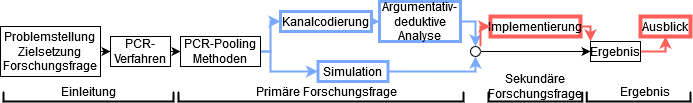
\includegraphics[height=.15\textwidth]{images/Untitled Diagram.drawio}
	%\caption{Geplanter Aufbau der Arbeit\footnotemark}
\end{figure}

\paragraph{Einleitung}
Die Einleitung beginnt mit einer Beschreibung der Problemstellung und Zielsetzung der Arbeit.
Hierauf folgen die Forschungsfragen, welche sich am Research Proposal orientieren.
Am Ende des Einleitungskapitels wird das PCR-Verfahren im Allgemeinen vorgestellt, um eine Grundlage für die Bearbeitung der Forschungsfragen zu schaffen.

\paragraph{Primäre Forschungsfrage}
Die Beantwortung der primären Forschungsfrage beginnt mit einer Aufbereitung der bisherigen Forschung zu PCR-Pooling-Verfahren.
Für die Validierung sind zwei Forschungsansätze denkbar:
\begin{itemize}
	\setlength{\itemsep}{-8pt}
	\item Qualitativer Ansatz:
				Die Disziplin der Kanalcodierung wird vorgestellt und auf Basis dieses wissenschaftlichen Frameworks die Pooling-Verfahren formalisiert.
				Hierauf erfolgt eine argumentativ-deduktive Analyse, welche die Methode durch theoretische und qualitative Ansätze überprüft.
	\item Quantitativer Ansatz:
				Die Pooling-Verfahren werden in Software nachgebaut und quantitativ anhand einer Simulation analysiert.
				Es werden unterschiedliche Grenzfälle getestet, um das Verhalten der Verfahren zu beobachten.
\end{itemize}

\paragraph{Sekundäre Forschungsfrage und Ausblick}
Die sekundäre Forschungsfrage ist die Implementierung der Methode im betrieblichen Umfeld.
Der Umfang dieser Forschung wird flexibel dem Ressourcenbedarf der primären Forschungsfrage angepasst.
Die Behandlung der Implementierung ist somit als eigenes Hauptkapitel denkbar.
Alternativ erfolgt eine Kürzung als Ausblick nach dem Ergebnis.

\paragraph{Ergebnis}
Die Arbeit endet mit einem Kapitel, in welchem die Erlebnisse zusammengefasst und Handlungsempfehlungen gegeben werden.
Es wird geprüft ob das Forschungsziel erreicht wurde und ob ein Optimierungspotenzial gegenüber den bisherigen Verfahren besteht.
Abhängig vom vorherigen Kapitel folgt ein Ausblick.